\RequirePackage{shellesc}
%\immediate\write18{cd ..; tex spath3_code.dtx}
\documentclass{article}
\thispagestyle{empty}
\usepackage[scale=.9,landscape]{geometry}
\usepackage{subcaption}
\usepackage{tikz}
\usetikzlibrary{
  knots,
  hobby,
  external,
  decorations.pathreplacing,
  shapes.geometric
}

\tikzset{
  external/figure name=knot,
  external/prefix=knotdiagrams/new-trefoil-,
  external/system call={pdflatex \tikzexternalcheckshellescape -halt-on-error -interaction=batchmode -jobname "\image" "\texsource" && pdftoppm -png -singlefile "\image.pdf" "\image"},
}

\tikzexternalize

\let\origtikzsetnextfilename\tikzsetnextfilename
\def\tikzsetnextfilename#1{%
  \origtikzsetnextfilename{#1}%
  \mysetlabel{#1}%
}

\newcommand{\mysetlabel}[1]{%
  \gdef\mynextlabel{#1}}

\newcommand{\autolabel}{%
  \label{fig:\mynextlabel}
  \global\let\mynextlabel\relax
}


\tikzset{
  use Hobby shortcut,
  trefoil/.style={
    draw,
    ultra thick,
    red
  },
  every picture/.style={
    execute at end picture={%
      \path ([shift={(-5pt,-5pt)}]current bounding box.south west)   ([shift={(5pt,5pt)}]current bounding box.north east);
    }
  }
}

\begin{document}
%\tikzset{external/force remake=true}

\begin{figure}
%% Trefoil
\subcaptionbox{Trefoil}[.25\linewidth][c]{%
  \tikzsetnextfilename{trefoil}
%\tikzset{external/export next=false}
  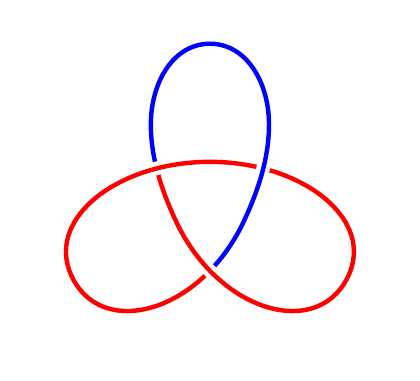
\begin{tikzpicture}[
    every trefoil component/.style={trefoil},
    trefoil component 3/.style={blue}
  ]
  
  \path[spath/save=trefoil] ([closed]90:2) .. (-.75,1) .. (210:.5) .. (330:2) .. (90:.5) .. (210:2) .. (330:.5) .. (.75,1);
  \tikzset{
    spath/knot={trefoil}{5pt}{2,4,6}
  }
\end{tikzpicture}
\autolabel
}%
%% Trefoil first twist
\subcaptionbox{Trefoil: First Twist}[.25\linewidth][c]{%
\tikzsetnextfilename{twist}
%\tikzset{external/export next=false}
\centering
  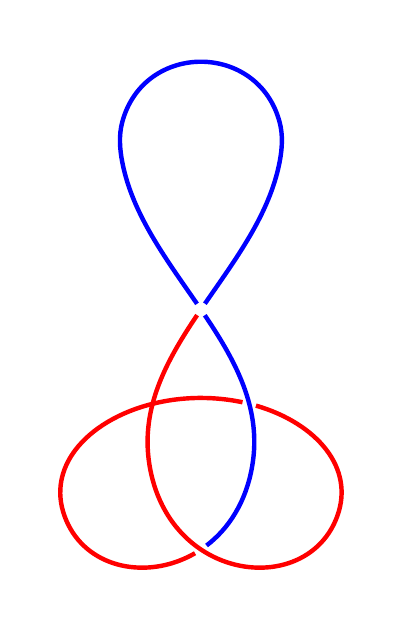
\begin{tikzpicture}[
    every first twist component/.style={trefoil},
    first twist component 3/.style={blue},
    first twist component 4/.style={blue},
    ]
  \path[spath/save=first twist] ([closed]1,4) .. (1,3.5) .. (210:.75) .. (330:2) .. (90:.5) .. (210:2) .. (330:.75)  .. (-1,3.5) .. (-1,4);
  \tikzset{
    spath/knot={first twist}{5pt}{3,5,7,8},
  }
\end{tikzpicture}
\autolabel
}%
%% Trefoil first move
\subcaptionbox{Trefoil: Move Over}[.25\linewidth][c]{%
\tikzsetnextfilename{first-over}
%\tikzset{external/export next=false}
\centering
  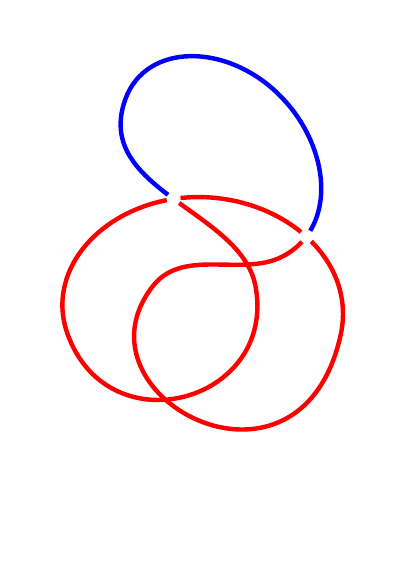
\begin{tikzpicture}[
    every first-over component/.style={trefoil},
    first-over component 4/.style={blue}
    ]
  \path[spath/save=first-over] ([closed]1,2) .. (1,0) .. (210:.75) .. (330:2) .. (90:.75) .. (210:2) .. (330:.75)  .. (-1,2);
  \tikzset{
    spath/knot={first-over}{5pt}{3,4,7,8},
  }
\end{tikzpicture}
\autolabel
}%
%% Trefoil slide round
\subcaptionbox{Trefoil: Slide Round}[.25\linewidth][c]{%
\tikzsetnextfilename{slide-round}
%\tikzset{external/export next=false}
\centering
  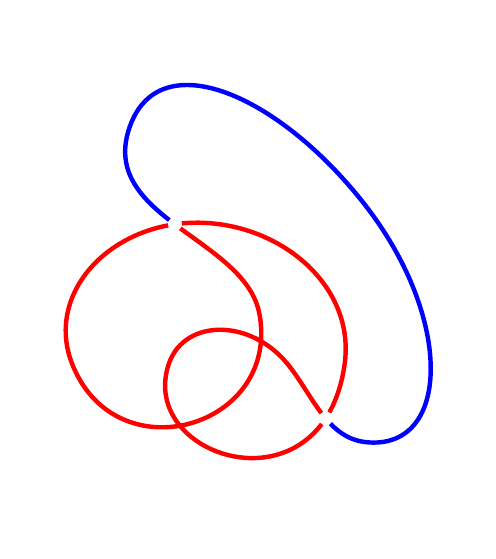
\begin{tikzpicture}[
    every slide-round component/.style={trefoil},
    slide-round component 4/.style={blue}
    ]
  \path[spath/save=slide-round] ([closed]2,1) .. (2,-2) .. (1,-1) .. (-.5,-1) .. (330:2) .. (0.25,.75) .. (210:2) .. (330:.75)  .. (-1,2);
  \tikzset{
    spath/knot={slide-round}{5pt}{3,4,7,8},
  }
\end{tikzpicture}
\autolabel
}
\end{figure}

\begin{figure}
%% Trefoil second move
\subcaptionbox{Trefoil: Second Move}[.25\linewidth][c]{%
\tikzsetnextfilename{second-move}
%\tikzset{external/export next=false}
\centering
  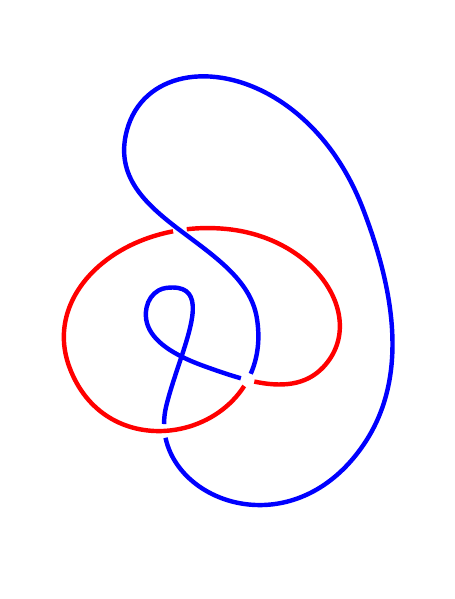
\begin{tikzpicture}[
    every second-move component/.style={trefoil},
    second-move component 1/.style={blue},
    second-move component 4/.style={blue}
    ]
  \path[spath/save=second-move] ([closed]2,1) .. (2,-2) .. (-.5,-1.5) .. (-.5,0) .. (-.75,-.25) .. (0,-1) .. (1.5,-1) .. (0.25,.75) .. (210:2) .. (330:.75)  .. (-1,2);
  \tikzset{
    spath/knot={second-move}{5pt}{3,4,6,8},
  }
\end{tikzpicture}
\autolabel
}%
%% Trefoil untwist
\subcaptionbox{Trefoil: Untwist}[.25\linewidth][c]{%
\tikzsetnextfilename{untwist}
%\tikzset{external/export next=false}
\centering
  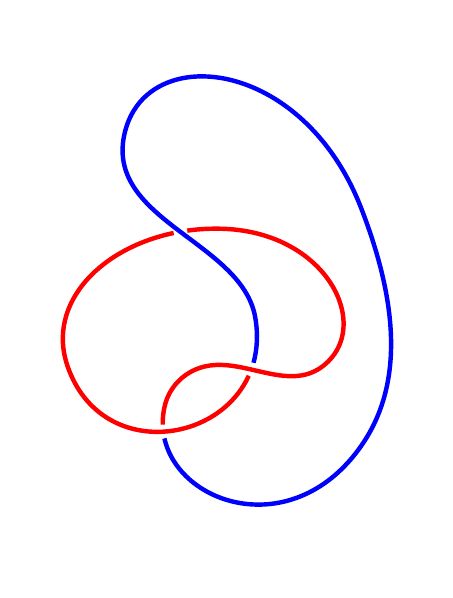
\begin{tikzpicture}[
    every untwist component/.style={trefoil},
    untwist component 3/.style={blue}
    ]
  \path[spath/save=untwist] ([closed]2,1) .. (2,-2) .. (-.5,-1.5) .. (0,-1) .. (1.5,-1) .. (0.25,.75) .. (210:2) .. (330:.75)  .. (-1,2);
  \tikzset{
    spath/knot={untwist}{5pt}{2,4,6},
  }
\end{tikzpicture}
\autolabel
}%
%% Trefoil slide round
\subcaptionbox{Trefoil: Slide Round Again}[.25\linewidth][c]{%
\tikzsetnextfilename{slide-again}
%\tikzset{external/export next=false}
\centering
  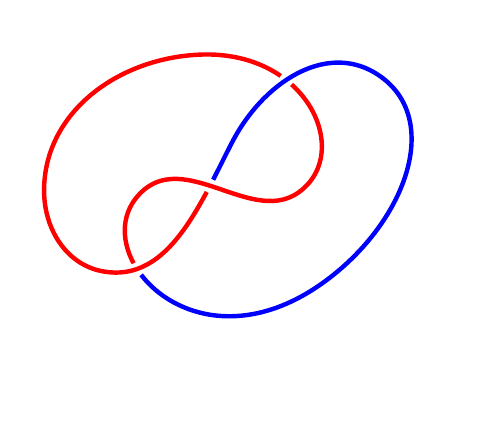
\begin{tikzpicture}[
    every slide-again component/.style={trefoil},
    slide-again component 3/.style={blue}
    ]
  \path[spath/save=slide-again] ([closed]2.5,.5) .. (2,-2) .. (-.5,-1) .. (1.5,-1) .. (0.25,.75) .. (210:2) .. (-1,-2) .. (330:.75);
  \tikzset{
    spath/knot={slide-again}{5pt}{2,4,6},
  }
\end{tikzpicture}
\autolabel
}%
%% Trefoil neaten
\subcaptionbox{Trefoil: Neaten}[.25\linewidth][c]{%
\tikzsetnextfilename{neaten}
%\tikzset{external/export next=false}
\centering
  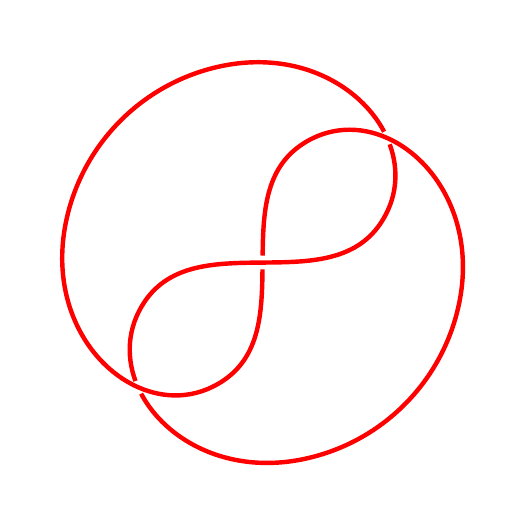
\begin{tikzpicture}[
    every neaten component/.style={trefoil}
  ]
  \path[spath/save=neaten] ([closed]0,2) .. (2,0) .. (-1,-1) .. (1,-3) .. (3,-1) .. (1,1) .. (0,-2) .. (-2,0);
  \tikzset{
    spath/knot={neaten}{5pt}{2,4,6},
  }
\end{tikzpicture}
\autolabel
}
\end{figure}

\end{document}
